\documentclass{article}

% Packages required to support encoding
\usepackage{ucs}
\usepackage[utf8x]{inputenc}
\usepackage{graphicx} 
% Packages required by code

% Packages always used
\usepackage{listings}
\usepackage{hyperref}
\usepackage{xspace}
\usepackage[usenames,dvipsnames]{color}
\hypersetup{colorlinks=true,urlcolor=blue}


\usepackage[framed,numbered,autolinebreaks,useliterate] {mcode}
\newcommand{\BigO}[1]{\ensuremath{\operatorname{O}\bigl(#1\bigr)}}

\usepackage{geometry}
\geometry{letterpaper,textwidth=350pt,textheight=680pt,tmargin=60pt,
            left=72pt,footskip=24pt,headsep=18pt,headheight=14pt}
\usepackage{amsmath}
\usepackage{amssymb}
\usepackage{textcase}
\usepackage{soul}

\newcommand{\mat}[1]{\boldsymbol{#1}}\renewcommand{\vec}[1]{\boldsymbol{\mathrm{#1}}}
\newcommand{\vecalt}[1]{\boldsymbol{#1}}

\newcommand{\conj}[1]{\overline{#1}}

\newcommand{\normof}[1]{\|#1\|}
\newcommand{\onormof}[2]{\|#1\|_{#2}}

\newcommand{\itr}[2]{#1^{(#2)}}
\newcommand{\itn}[1]{^{(#1)}}

\newcommand{\eps}{\varepsilon}
\newcommand{\kron}{\otimes}

\DeclareMathOperator{\diag}{diag}
\DeclareMathOperator{\trace}{trace}
\DeclareMathOperator{\tvec}{vec}

\newcommand{\prob}{\mathbb{P}}
\newcommand{\probof}[1]{\prob\left\{ #1 \right\}}

\newcommand{\pmat}[1]{\begin{pmatrix} #1 \end{pmatrix}}
\newcommand{\bmat}[1]{\begin{bmatrix} #1 \end{bmatrix}}
\newcommand{\spmat}[1]{\left(\begin{smallmatrix} #1 \end{smallmatrix}\right)}
\newcommand{\sbmat}[1]{\left[\begin{smallmatrix} #1 \end{smallmatrix}\right]}

\newcommand{\RR}{\mathbb{R}}
\newcommand{\CC}{\mathbb{C}}

\providecommand{\eye}{\mat{I}}
\providecommand{\mA}{\ensuremath{\mat{A}}}
\providecommand{\mB}{\ensuremath{\mat{B}}}
\providecommand{\mC}{\ensuremath{\mat{C}}}
\providecommand{\mD}{\ensuremath{\mat{D}}}
\providecommand{\mE}{\ensuremath{\mat{E}}}
\providecommand{\mF}{\ensuremath{\mat{F}}}
\providecommand{\mG}{\ensuremath{\mat{G}}}
\providecommand{\mH}{\ensuremath{\mat{H}}}
\providecommand{\mI}{\ensuremath{\mat{I}}}
\providecommand{\mJ}{\ensuremath{\mat{J}}}
\providecommand{\mK}{\ensuremath{\mat{K}}}
\providecommand{\mL}{\ensuremath{\mat{L}}}
\providecommand{\mM}{\ensuremath{\mat{M}}}
\providecommand{\mN}{\ensuremath{\mat{N}}}
\providecommand{\mO}{\ensuremath{\mat{O}}}
\providecommand{\mP}{\ensuremath{\mat{P}}}
\providecommand{\mQ}{\ensuremath{\mat{Q}}}
\providecommand{\mR}{\ensuremath{\mat{R}}}
\providecommand{\mS}{\ensuremath{\mat{S}}}
\providecommand{\mT}{\ensuremath{\mat{T}}}
\providecommand{\mU}{\ensuremath{\mat{U}}}
\providecommand{\mV}{\ensuremath{\mat{V}}}
\providecommand{\mW}{\ensuremath{\mat{W}}}
\providecommand{\mX}{\ensuremath{\mat{X}}}
\providecommand{\mY}{\ensuremath{\mat{Y}}}
\providecommand{\mZ}{\ensuremath{\mat{Z}}}
\providecommand{\mLambda}{\ensuremath{\mat{\Lambda}}}
\providecommand{\mPbar}{\bar{\mP}}

\providecommand{\ones}{\vec{e}}
\providecommand{\va}{\ensuremath{\vec{a}}}
\providecommand{\vb}{\ensuremath{\vec{b}}}
\providecommand{\vc}{\ensuremath{\vec{c}}}
\providecommand{\vd}{\ensuremath{\vec{d}}}
\providecommand{\ve}{\ensuremath{\vec{e}}}
\providecommand{\vf}{\ensuremath{\vec{f}}}
\providecommand{\vg}{\ensuremath{\vec{g}}}
\providecommand{\vh}{\ensuremath{\vec{h}}}
\providecommand{\vi}{\ensuremath{\vec{i}}}
\providecommand{\vj}{\ensuremath{\vec{j}}}
\providecommand{\vk}{\ensuremath{\vec{k}}}
\providecommand{\vl}{\ensuremath{\vec{l}}}
\providecommand{\vm}{\ensuremath{\vec{l}}}
\providecommand{\vn}{\ensuremath{\vec{n}}}
\providecommand{\vo}{\ensuremath{\vec{o}}}
\providecommand{\vp}{\ensuremath{\vec{p}}}
\providecommand{\vq}{\ensuremath{\vec{q}}}
\providecommand{\vr}{\ensuremath{\vec{r}}}
\providecommand{\vs}{\ensuremath{\vec{s}}}
\providecommand{\vt}{\ensuremath{\vec{t}}}
\providecommand{\vu}{\ensuremath{\vec{u}}}
\providecommand{\vv}{\ensuremath{\vec{v}}}
\providecommand{\vw}{\ensuremath{\vec{w}}}
\providecommand{\vx}{\ensuremath{\vec{x}}}
\providecommand{\vy}{\ensuremath{\vec{y}}}
\providecommand{\vz}{\ensuremath{\vec{z}}}
\providecommand{\vpi}{\ensuremath{\vecalt{\pi}}}

\sodef\allcapsspacing{\upshape}{0.15em}{0.65em}{0.6em}%

\makeatletter
\def\maketitle{%
\par
\hrule height 0.75pt\vspace{1ex}
\par\noindent
\begin{minipage}{0.5\textwidth}
\scshape
purdue university $\cdot$ CS 580 \\
Introduction to the Analysis of Algorithms
\end{minipage}
\begin{minipage}{0.5\textwidth}
\raggedleft
\MakeTextUppercase{\allcapsspacing{\@title}}\\[0.2ex]
\textit{\@author}\\[0.2ex]
\textit{\@date}
\end{minipage}
\par\vspace{1ex}
\hrule height 1pt
\vspace{2ex}
\par
}
\makeatother

\author{Jun Cheng}
\title{Lecture Notes}
% auto generate a title
\AtBeginDocument{\maketitle}


\title{Homework}



\begin{document} 



\hypertarget{problem_0_homework_checklist_2}{}
\subsection*{{Problem 0: Homework checklist}}
\label{problem_0_homework_checklist_2}

\checkmark	I didn't talk with any one about this homework. \newline
\checkmark 	Source-code are included at the end of this document. 


\hypertarget{problem_0_homework_checklist_2}{}
\subsection*{{Problem 1: The Cholesky Factorization}}
\label{}
\begin{enumerate} 
\item 
Here is my implementation of Cholesky decomposition in Matlab: 
\begin{lstlisting}
function L = cholesky(A)
n = size(A); 
n = n(1); 
L = zeros(n,n);
%L(1,1) = sqrt(A(1,1)); 
for i=(1:n)
    sum1 =0;     
    for j=(1:i) 

        if i==j
            L(j,j) = sqrt(A(j,j)-sum1); 
        else 
            sum2 = 0; 
            for k = (1:j-1) 
                sum2 = sum2 + L(i,k)*L(j,k); 
            end 
            
            L(i,j) = 1/L(j,j)*(A(i,j)-sum2); 
        end 
        sum1= sum1 + L(i,j)^2;   
    end 
end 
end 
\end{lstlisting} 
\item 
Cholesky factorization is unique if $\mA$ is positive definite and the decomposition need not be unique when $\mA$ is positive semidefinite.  

\item 
Both have the same result. 
\item 
For each size of the matrices I repeated 10 times. The comparison result is shown.   Obviously the the Cholesky factorization has better performance as the growth of matrix size. 
\begin{figure} 
\centering 
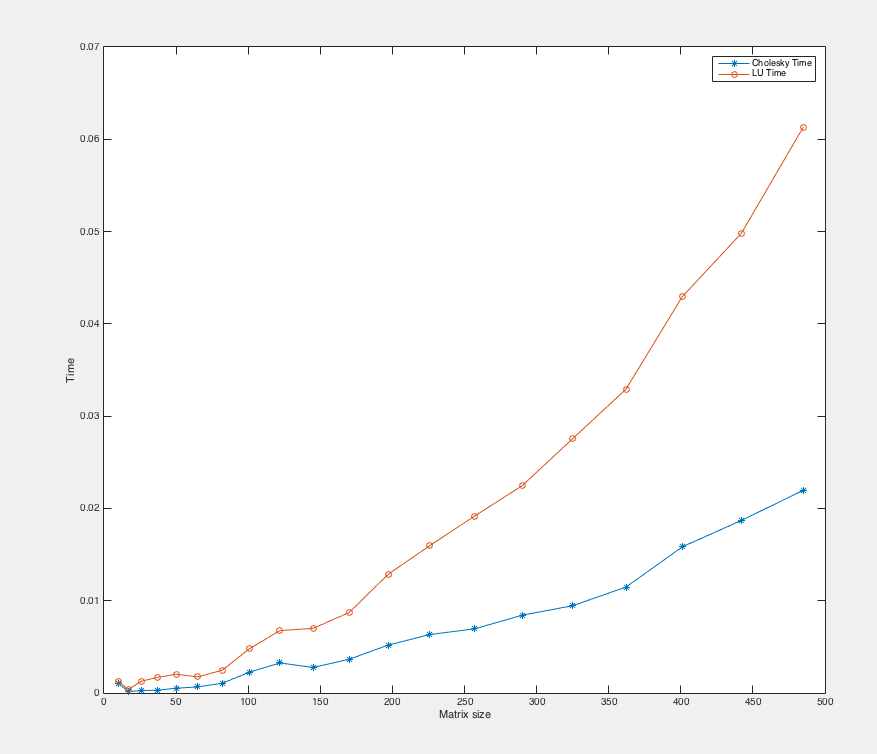
\includegraphics[width=0.8\textwidth]{luVScholesky}
\caption{Performance comparison between LU decomposition and Cholesky factorization}
\end{figure}

\item 
Since $\mA$ is positive definite, and assume an vector $\vv = \bmat{x_0\\ \vx}, \\ $then \\
\begin{align*} 
\vv_T\mA\vv>0 \\
\bmat{x_0 & \vx}\bmat{\alpha & \vb_T\\ \vb & \mC} \bmat{x_0\\ \vx} = \alpha x_0^2 + x_0(\vx^T\vb+\vb^T\vx) + \vx^T\mC\vx >0  
\end{align*}
Then 
\begin{align*}
\vx^T(\mC-\frac{\vb\vb^T}{\alpha})\vx &= \vx^T\mC\vx - \frac{\vx_T\vb\vb^T\vx}{\alpha} \\
& > -\alpha x_0^2 - x_0(\vx^T\vb+\vb^T\vx) - \frac{\vx^T\vb\vb^T\vx}{\alpha} \\
& = -\frac{1}{\alpha} \left[x_0^2 + \frac{\vx^T\vb+\vb^T\vx)x_0}{\alpha}+\frac{\vx^T\vb\vb^T\vx}{\alpha^2}\right]\\
& = -\frac{1}{\alpha}\left(x_0+\frac{\vx^T\vb}{\alpha}\right)\left(x_0+\frac{\vb^T\vx}{\alpha}\right) \\
& =  -\frac{1}{\alpha}\left\|x_0+\frac{\vb^T\vx}{\alpha}\right\|^2 
\end{align*} 
Because $\vx^T(\mC-\frac{\vb\vb^T}{\alpha})\vx > -\frac{1}{\alpha}\left\|x_0+\frac{\vb^T\vx}{\alpha}\right\|^2$ holds for any vector $\vx$. Therefore \begin{align} 
\vx^T(\mC-\frac{\vb\vb^T}{\alpha})\vx > 0 
\end{align} 
So $\mC-\frac{\vb\vb^T}{\alpha}$ is positive definite. 

\item  
The base case is that $C$ is a $1\times1$. 

\item 
\end{enumerate}

\hypertarget{}{}
\subsection*{{Problem 2: Stability analysis}}
\label{}
\begin{enumerate} 
\item 

\item 

\end{enumerate} 

\hypertarget{}{}
\subsection*{{Problem 3: Backwards stability}}
\label{}

\begin{align*}
fl(x_i) = x_i(1+\epsilon_{ix}) \\
fl(y_i) = y_i(1+\epsilon_{iy}) \\
\end{align*} 
where $|\epsilon_{ix}|, |\epsilon_{iy}|\leq\epsilon_{machine} $ \\
\begin{align*}
\alpha &=\vx^T\vy \\
& = \bmat{x_1 & x_2 & .. & x_n}\bmat{y_1 \\ y_2 \\ .. \\ y_n} \\
& = \sum_{i=1}^nx_i y_i \\ 
\end{align*} 
Then \begin{align*} 
fl(\vx^T\vy) & = \sum_{i=1}^nfl(x_i)\times fl( y_i) \\
& = \left[fl(x_1)\times fl(y_1)+ fl(x_2)\times fl(y_2) + ... + fl(x_n)\times fl(y_n)\right] (1+\epsilon_{addition})\\
& = \left[x_1y_1(1+\epsilon_{1x})(1+\epsilon_{1y}) + ... + x_ny_n(1+\epsilon_{nx})(1+\epsilon_{ny})\right](1+\epsilon_{addition}) \\ 
& = \left[x_1y_1 + x_2y_2 + ... +x_ny_n\right](1+\epsilon_1)(1+\epsilon_2)(1+\epsilon_3)\\
& = \left[x_1y_1 + x_2y_2 + ... +x_ny_n\right](1+\BigO{\epsilon_{machine}^2})
\end{align*}
Therefore the inner product is backwards stable. \\

\end{document}
